% --- [ Recovery of 2-way Conditionals ] ---------------------------------------

\subsection{Recovery of 2-way Conditionals}
\label{sec:recovery_of_2way_conditionals}

The control flow recovery results of the Hammock method, the Interval method, and for comparison the theoretical optimum when recovering \textit{2-way conditionals} (e.g. \texttt{if-else} statements) from the combined test programs of Coreutils and SQLite are presented in figure \ref{fig:total_results_2way}.

The \textbf{Hammock method} correctly recovered $46.68\%$ of the 2-way conditionals present in the test programs (\textit{true positives}). On average, for every $10$ 2-way conditionals of the original source code, the Hammock method recovered $3.9$ 2-way conditionals that were \textit{not} present of the original source code (\textit{false positives}).

The \textbf{Interval method} correctly recovered $74.84\%$ of the 2-way conditionals present in the test programs (\textit{true positives}). On average, for every $10$ 2-way conditionals of the original source code, the Interval method recovered $5.0$ 2-way conditionals that were \textit{not} present of the original source code (\textit{false positives}).

Note, at this level of comparison, \textit{if} statements and \textit{if-else} statements are both regarded as 2-way conditionals. While the Hammock method distinguishes 1-way conditionals from 2-way conditionals at the control flow recover stage, the Interval method distinguishes 1-way conditionals from 2-way conditionals at the code generation state. For this reason, no distinction is made between 1-way and 2-way conditionals during the evaluation.

\begin{figure}[htbp]
	\centering
	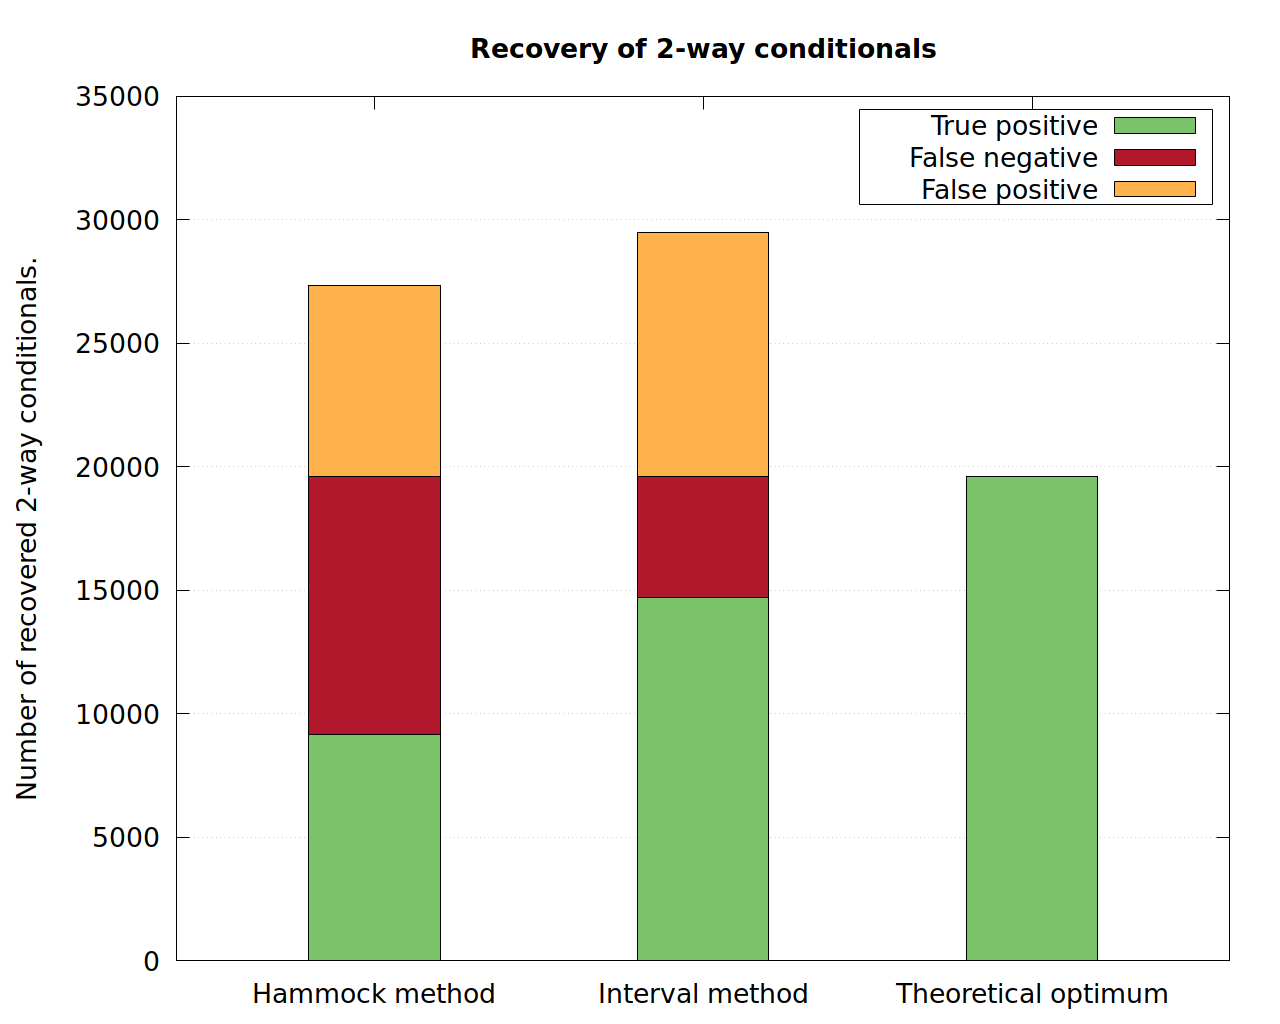
\includegraphics[width=\textwidth]{inc/5_results/results_2-way.png}
	\caption{Comparison of control flow recovery results for each method when recovering \textit{2-way conditionals}. The data is based on the combined test programs of Coreutils and SQLite.}
	\label{fig:total_results_2way}
\end{figure}
